\shorthandoff{'}
\begin{markdown*}{%
  hybrid,
  definitionLists,
  footnotes,
  inlineFootnotes,
  hashEnumerators,
  fencedCode,
  citations,
  citationNbsps,
  pipeTables,
  tableCaptions,
}

\chapter{Jaculus-dcore}

To make porting Jaculus to different platforms easier, the core functionality of a Jaculus device (e.g., communication, control protocol, JavaScript runtime) is implemented in the Jaculus-dcore library in a platform-independent way. The library requires C++20 and POSIX support to be available on the target platform.

Jaculus-dcore uses the Jaculus-machine library for the JavaScript runtime and the Jaculus-link library for communication.

\section{Architecture}

The Jaculus-dcore library is centered around the `Device` class, which is used to define a Jaculus device and which bundles all of the core functionality of the library.

\subsection{Device class}

The `Device` class is the entry point for defining a Jaculus device. It is a template parametrized by the Machine type used for the JavaScript runtime. The Machine type must implement the `evalFile` method, which is used to run the code uploaded to the device.

The `Device` class exposes a `Router` object from Jaculus-link, which is used to connect the device to the communication interface. `Device` also exposes an interface for controlling the internal Machine instance from C++ code.

Three services are also part of the `Device` class and expose functionality over the communication channel (or channels):

  - Controller --- service for controlling and monitoring the device
  - Uploader --- service for uploading code/data to the device
  - Logger --- service for logging messages from the device

The services use separate channels provided by the `Router` object. Other channels are also reserved for the standard input and output of the JavaScript instance.

The `Device` implements a locking mechanism to prevent multiple clients from accessing the device simultaneously. The lock is paired with a timeout, which is continuously reset while the client communicates with the devices. If the timeout expires, the lock is released, and other clients can access the device. The lock is exposed to the client via the Controller service.


\section{Implementation}

\subsection{Controller service}

The Controller service is implemented in the `Controller` class. It uses a *PacketCommunicator* interface to communicate with the client.

The first byte of each packet is used to specify the command to be executed. The rest of the packet is used to transmit command-specific data. The packet structure of the protocol is shown in a diagram in Figure \ref{fig:controller-protocol}.

The service exposes the following functionality:

  - accessing the device lock,
  - controlling the internal Machine instance,
  - using the Machine instance's standard input and output, and
  - monitoring the device status.

\begin{figure}[!ht]
    \centering
    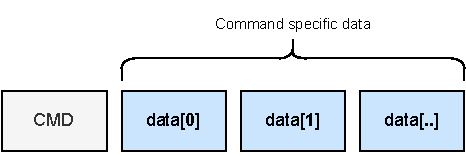
\includegraphics[width=0.5\textwidth]{img/controller-packet}
    \caption{Controller protocol packet structure}
    \label{fig:controller-protocol}
\end{figure}

\subsection{Uploader service}

The Uploader service is implemented in the `Uploader` class. Similarly to the Controller service, it uses a *PacketCommunicator* interface to communicate with the client. The first byte of each packet is used to specify the command to be executed. The rest of the packet is used to transmit command-specific data. The packet structure of the protocol is shown in a diagram in Figure \ref{fig:uploader-protocol}.

The service provides the following functionality:

  - listing files and directories,
  - creating and deleting directories, and
  - writing, reading, and deleting files.

Most commands are processed in a single packet, but writing files requires the data to be sent in multiple packets. When writing a file, an internal state is set to specify what operation should be performed when data is received and when the transmission is finished. To prevent overflow of the receiving buffer, the command implements, admittedly relatively inefficient, flow control --- the client must acknowledge each packet before the next one is sent.

Commands for reading a file and listing a directory might also split the data into multiple packets. For simplicity, no flow control is implemented when transmitting data to the client, as the client is expected to be a much more powerful device that can handle the transmission speed.

\begin{figure}[!ht]
    \centering
    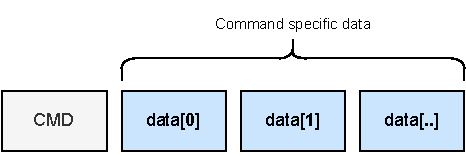
\includegraphics[width=0.5\textwidth]{img/controller-packet}
    \caption{Uploader protocol packet structure}
    \label{fig:uploader-protocol}
\end{figure}

\subsection{Filesystem access}

The Uploader service provides access to the filesystem of the device. Unfortunately, because `std::filesystem` is not yet fully implemented in ESP-IDF, the implementation has to, in some cases, rely on the POSIX filesystem API to run on the ESP platform.


\section{Usage}

\subsection{Creating a new device}

To create a new device, an instance of the `Device` class must be created. The class is templated by the Machine type used for the JavaScript runtime. The definition of a Machine type is described in Section \ref{sec:machine-usage}.

The `Device` must be connected to a communication interface. The object exposes a `Router` object from Jaculus-link, which should be used to connect the device to a data link. Definition and binding of a data link are described in Section \ref{sec:link-usage}.

After the device is initialized, the `Device::start` method must be called to start the provided services.

An example of a device definition can be seen in Jaculus-esp32 in the `main.cpp` file.

\subsection{Controlling the device}

To control the device, the user can use the Jaculus-tools application, which provides a command-line interface for managing the device. The application is described in the following chapter in more detail.


\shorthandon{'}
\end{markdown*}
